%%%%%%%%%%%%%%%%%%%%%%%%%%%%%%%%%%%%%%%%%%%%%%%%%%%%%%%%%%%%%%%%%%%%%%%%%%%%%%%%
%2345678901234567890123456789012345678901234567890123456789012345678901234567890
%        1         2         3         4         5         6         7         8

\documentclass[letterpaper, 10 pt, conference]{ieeeconf}  % Comment this line out
                                                          % if you need a4paper
%\documentclass[a4paper, 10pt, conference]{ieeeconf}      % Use this line for a4
                                                          % paper

\IEEEoverridecommandlockouts                              % This command is only
                                                          % needed if you want to
                                                          % use the \thanks command
\overrideIEEEmargins
% See the \addtolength command later in the file to balance the column lengths
% on the last page of the document
\usepackage{hyperref}
\usepackage{listings}
\usepackage{biblatex}
\bibliography{paper}
\usepackage{float}
\let\proof\relax
\let\endproof\relax
\usepackage{amsmath, amsthm, amssymb}
\usepackage{graphicx}
% The following packages can be found on http:\\www.ctan.org
%\usepackage{graphics} % for pdf, bitmapped graphics files
%\usepackage{epsfig} % for postscript graphics files
%\usepackage{mathptmx} % assumes new font selection scheme installed
%\usepackage{times} % assumes new font selection scheme installed
%\usepackage{amsmath} % assumes amsmath package installed
%\usepackage{amssymb}  % assumes amsmath package installed
\lstset{
%  basicstyle=\ttfamily,
  columns=fullflexible,
  frame=single,
  breaklines=true,
  basicstyle=\small
}

\title{\LARGE \bf
Object Detection-Based Behaviour using Deep-Learning on Thymio
}


\author{Francesco Saverio Zuppichini$^{1}$ and Alessia Ruggeri$^{2}$% <-this % stops a space
\thanks{$^{1}$Francesco Saverio Zuppichini, \href{mailto:zuppif@usi.ch}{zuppif@usi.ch} , AI master student at Università della Svizzera Italiana }%
\thanks{$^{2}$Alessia Ruggeri, \href{mailto:ruggea@usi.ch}{ruggea@usi.ch} , AI master student at Università della Svizzera Italiana }%
}

\begin{document}


\maketitle
\thispagestyle{empty}
\pagestyle{empty}


%%%%%%%%%%%%%%%%%%%%%%%%%%%%%%%%%%%%%%%%%%%%%%%%%%%%%%%%%%%%%%%%%%%%%%%%%%%%%%%%
\begin{abstract}
The ability to classify objects in both space and domain is encoded in an enormous variety of species on the planet. Recently, deep learning approaches have been developed to make machines able to mimic the same task with interesting results. With this paper, we propose a minimal architecture to archive the same goal using a cheap two-wheels robot, the Thymio, with a mounted frontal camera in order to make it moves based on the objects detected in the surrounding. 
\end{abstract}

\section{Introduction}
Finding objects in space by identifying their identity and their coordinates is a basic task that almost every animal is able to accomplish. The ability to solve this problem is extremely important in robotics, where a machine needs to act based on its surrounding.  We implemented an architecture, running on ROS, that is able to find selected target objects through YOLO, a real-time object detection model,  by only using a cheap camera.

Specifically, our robot will wait for a user-specified class, e.g. \emph{dog}, and, when found, it moves towards the object by keeping it in the middle of its view. We also implemented a PID-based algorithm to avoid obstacles and properly stop in front of the founded item.

The paper is structured as follows: we will first describe the architecture by showing each individual part of the topology and how they interact; then, we will discuss the challenges during the development process and, finally, we will show the results.

\section{Architecture overview}
We used the Robotic Operating System,\cite{ROS}, since it is \emph{de facto} the state of the art. Our architecture is composed by:
\begin{enumerate}
	\item A robot with a mounted camera and with a ROS node running on the on-board computer;
	\item A web server running the Object Detection model;
	\item A ROS node running on a local machine that controls the robot.
\end{enumerate}
As a robot, we used the \emph{MightyThymio} \cite{guzzi2018eaai}, which is a robot developed on top of the Thymio, a small mass-produced mobile robot usually used in primary and secondary education. The MightyThymio has a powerful Odroid C1 on board, a 1GB quad-core ARM Linux machine, with a HD camera mounted on top. The authors also implemented a ROS node to communicate with it and open-sourced the code.

\subsection*{The MightyThymio Robot}

In our project, the MightyThymio has the same configuration proposed in \cite{guzzi2018eaai}. Briefly, the onboard computer exposes the Thymios sensors through ROS. Thus, another ROS node can publish and subscribe to it in order to communicate with its sensors. For example, we can subscribe to the \emph{camera sensors} to get information from the proximity sensors to avoid hitting obstacles. Also, we can simply subscribe to the camera's topic to get both compressed and uncompressed images. 
\begin{figure}[H]
\centering
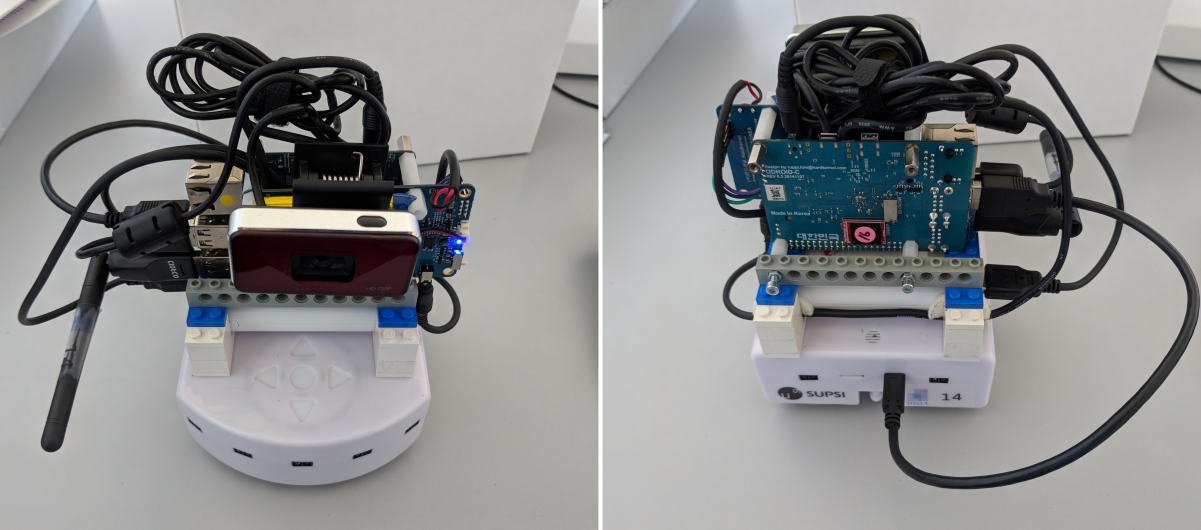
\includegraphics[width=\linewidth]{assembled_myt}	
\caption{The MightyThymio}
\end{figure}

\subsection*{Local ROS node}
We created a new ROS node to communicate with the running node on the MightyThymio, in order to control it accordingly with a specified behaviour based on the object detected by the model. The user specifies a set of target classes, for example \emph{dog} and \emph{cat}. Then our node, after having subscribed to the camera topic of the MightyThymio, sends the fetched image to the model hosted on a Web  Server through an HTTP request and gets as response the detected classes and their bounding boxes. In case there is no target object, the robot enters in \texttt{exploration} mode and starts spinning around. When one or more of the target classes are found simultaneously, the robot will go towards the target with the biggest bounding box area while keeping it in the center of the camera in order to follow it. In addition, we have an obstacle-avoiding algorithm in order to properly stop the Thymio before it hits the target.

\subsection*{Object Detection REST-API Web Server}
We used pre-trained Keras implementation\footnote{https://github.com/qqwweee/keras-yolo3} of YOLO\cite{DBLP:conf/cvpr/RedmonDGF16} model, the state-of-the-art real-time object detection model, with TensorFlow\cite{tensorflow2015-whitepaper} backend to predict the classes in the image and their bounding boxes. A bounding box is a rectangle in which the predicted class is contained. For example, in the following picture we can see the bounding boxes for a \emph{dog}, a \emph{bicycle} and a \emph{truck}. Each box is labelled with the class name and its score.
\begin{figure}[H]
\centering
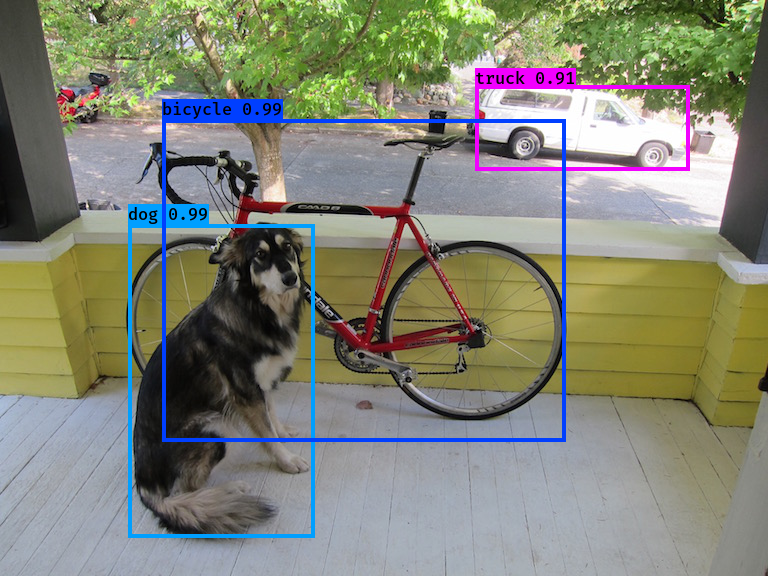
\includegraphics[width=\linewidth]{images/yolo-example}
\label{fig: yolo-example}
\caption{Yolo Prediction Example}
\end{figure}
The model was trained on the COCO(Common Object in Context)\cite{COCO} Dataset, that contains 80 classes. 

On top of that, we built a REST-API Web Server using Python3 and Flask\footnote{http://flask.pocoo.org/}, a micro-framework to create Web Servers, in order to make the model accessible from the Web. We decided to decouple the logic behind the robot behavior and the model in order to make our architecture more scalable. For instance, if needed, we can deploy our model in the cloud while keeping the running ROS code intact. 

The following endpoints are available:
\begin{lstlisting}
GET /model
POST /prediction  --image --size --compress
\end{lstlisting}
Each of them returns a JSON serialised response. The \texttt{/model} endpoint is used to get information about the model. This information are the classes that can be predicted and the colour associated to each one of them. It follows a response sample:
\begin{lstlisting}
{
    "classes": [ 
    "person", 
    "bicycle", 
    "car", 
    "motorbike", 
    "aeroplane", ... ]
    "colors": [[255, 38, 0], [0, 63, 255], ... ]   
 }
\end{lstlisting}
The client can get a prediction by sending an image to \texttt{/prediction}. It is also possible to specify if the image is compressed or not and if the server should resize it before feeding it to the model. In our case, we send a compressed image directly taken from the MightyThymio after subscribing to the \texttt{/camera/compressed} topic and we define the resized size to (190,190). The small size is due to the low computational power since we had no access to a GPU. By sanding the same image showed in Figure \ref{fig: yolo-example} we get the following response.
\begin{lstlisting}
{'res': [{'boxes': [96.21580505371094,
                    219.6134033203125,
                    437.66387939453125,
                    594.16748046875],
          'class': 'bicycle',
          'class_idx': 1,
          'score': 0.48406994342803955}, ...
         ]
 'time': 0.174407958984375}
\end{lstlisting}
For each detected class we return the bounding boxes, the \texttt{boxes} key of the JSON, the class name, its index, and the score, that is the confidence of the model. Each box is composed by the top, left, bottom and right offsets of the bounding box with respect to the left and the top of the image. In the above example, the bicycle's bounding starts at $96$ pixels from the left and at $219$ pixels from the top.

%
%\subsection{YOLO: Real-Time Object Detection}
%
%YOLO \cite{DBLP:conf/cvpr/RedmonDGF16} is a trained model for real-time object detection. While prior work on object detection repurposes classifiers to perform detection, YOLO handle the object detection as a regression problem to spatially separated bounding boxes and associated class probabilities. YOLO avoids resorting to complex pipelines that are slow and hard to optimize; instead, it uses a single convolutional neural network that simultaneously predicts multiple bounding boxes and class probabilities for those boxes. Using YOLO, You Only Look Once at an image to predict what objects are present and where they are.
%
%YOLO neural network uses features from the entire image to predict each bounding box simultaneously across all classes. The convolutional neural network contains 24 convolutional layers, that extract features from the image, followed by 2 fully connected layers, whose aim is to predict the output probabilities and coordinates. The system divides the input image into an $S \times S$ grid; if the centre of an object falls into a grid cell, that grid cell is responsible for detecting that object. Each grid cell predicts $B$ bounding boxes and confidence scores for those boxes. These confidence scores reflect how confident the model is that the box contains an object and also how accurate it thinks the box is that it predicts. There is also a fast version of YOLO, designed with a neural network with fewer convolutional layers and fewer filters in those layers.
%
%YOLO is extremely fast, it reason globally about the image when making predictions, it learns generalizable representations of objects and it is open source. YOLO still lags behind other detection systems in accuracy; while it can quickly identify object in images, it struggles to precisely localize some objects, especially small ones. However, it is still the state-of-the-art model for object detection in real-time.
%
%For our project, we used the third version of YOLO, or YOLOv3 \cite{Yolo3}, which has been improved by making it a little bigger than before, but more accurate.

\section{Implementation}
We designed our ROS node to find a specified object and follow it until it is close enough. In addition, we also implemented a PID-based algorithm to avoid obstacles and to stop before crashing into the target object. From a high-level view, the robot can be represented as a state machine with three states.
\begin{figure}[H]
\centering
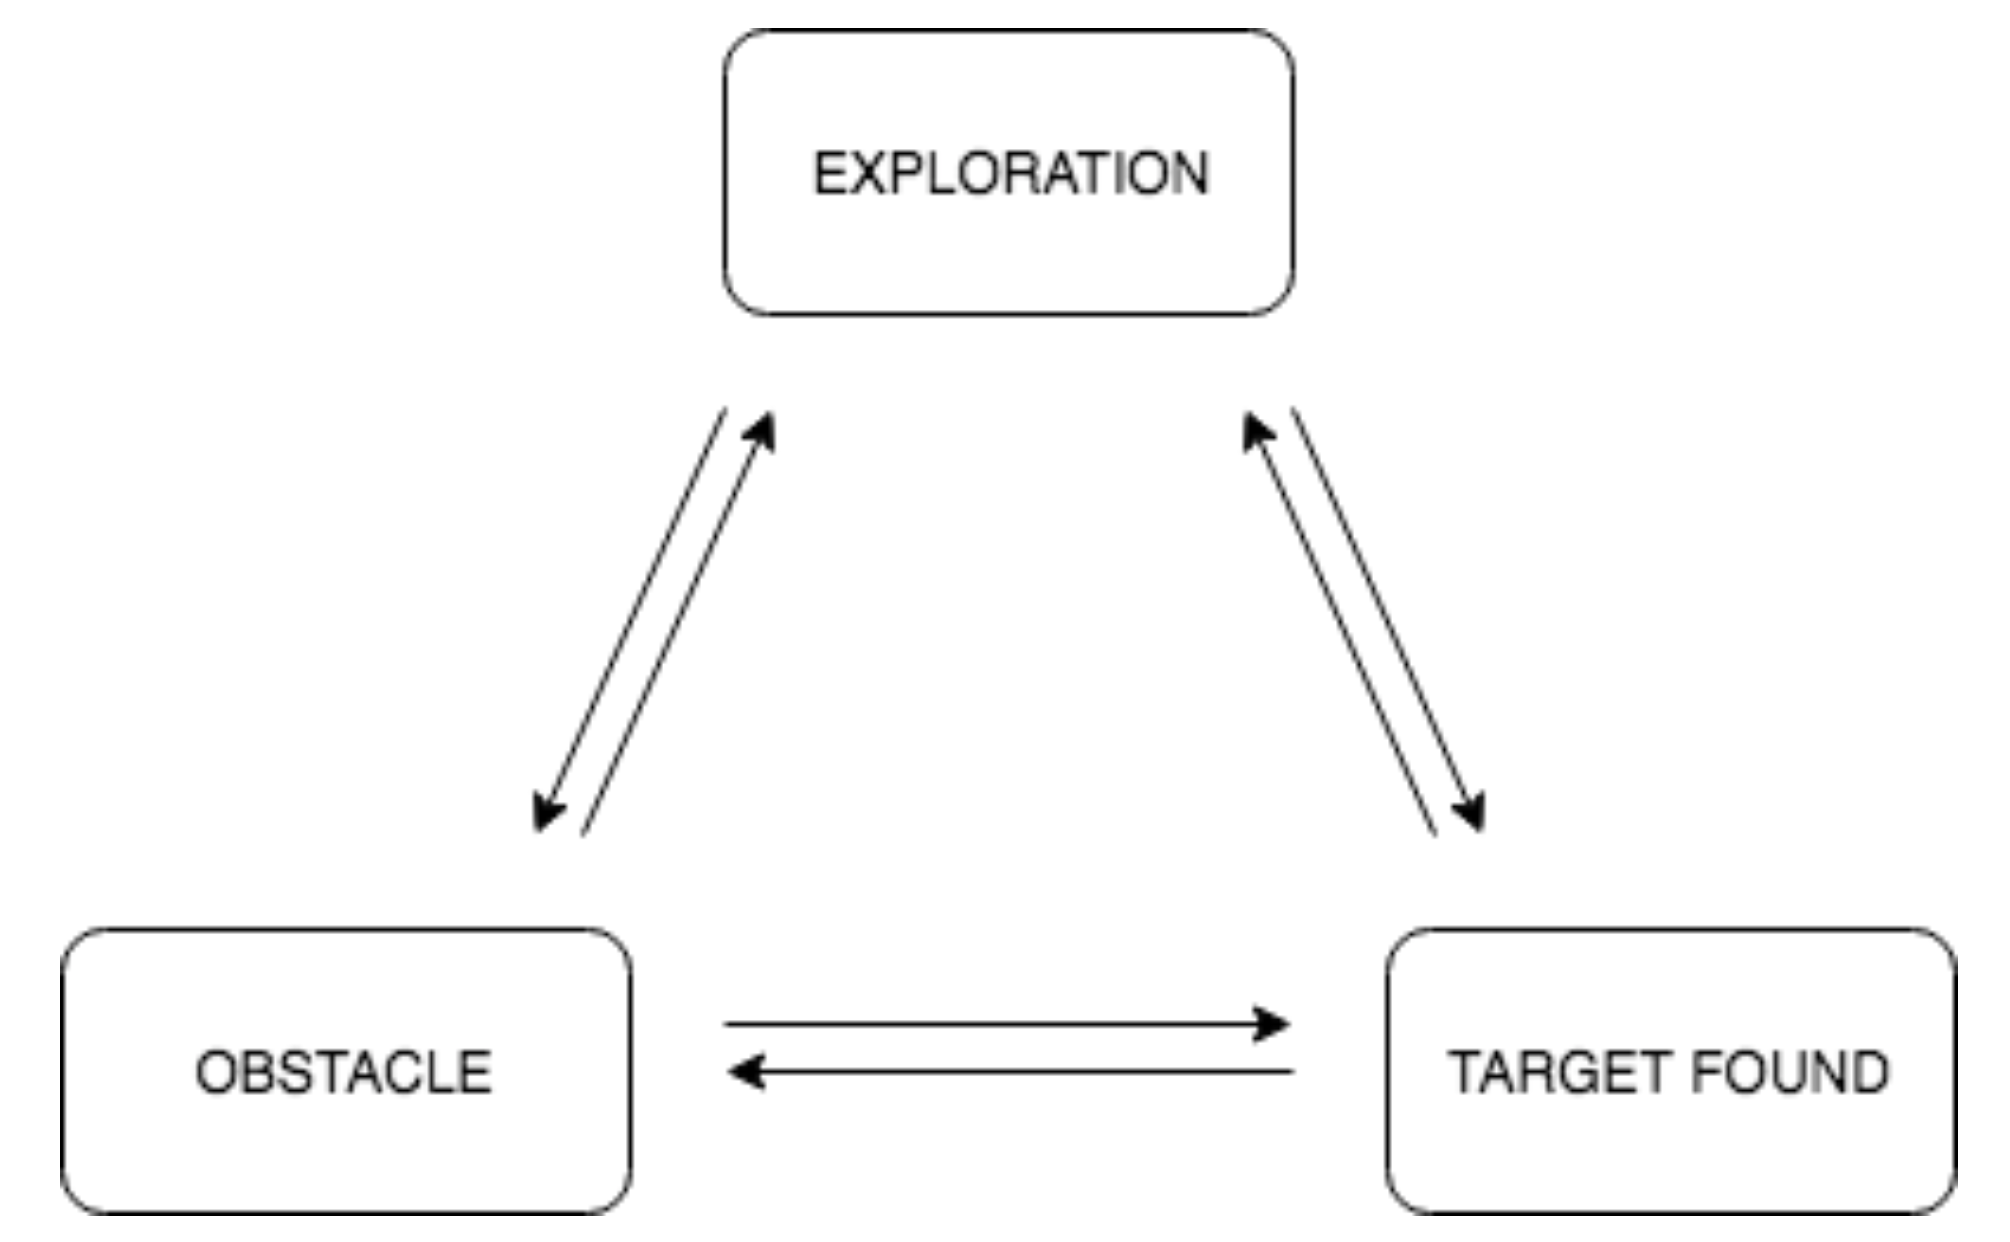
\includegraphics[width=\linewidth]{images/state}
\caption{State Machine}
\end{figure}
Thus, at any time, the machine can be \textbf{only} in one of the three states: \emph{exploration}, \emph{obstacle} and \emph{target found}. 

\paragraph{Exploration} The robot starts to spin on itself with a fixed angular velocity in order to scan the surrounding until it finds the target or it detects an obstacle.
\paragraph{Target Found} When a target object is found, the robot starts moving towards it by keeping its bounding box centred in the camera's centre. We used a Proportional Integral Derivative (PID) controller to select the correct angular velocity. Given the camera's image and the bounding box, we define the error at time $t$ as:
\begin{equation}
e_t =  (l_b + \frac{w_b}{2}) - \frac{w_c}{2}
\end{equation}
Where, $w_c$ is the camera's image width, in our case 640, $l_b$ and $w_b$ are the left component and the width of target's bounding box respectively. To find $w_b$ we need to just subtract the left and right component of the box. We are not taking the absolute value of the error since the sign is used to decide in which direction to turn. Before feeding the error to the PID controller we normalize it between zero and one by dividing by $w_c$, otherwise, we should have defined a very small proportional parameter for the PID. 

After computing the error for the current box, we pass it as parameter to a PID with a proportional parameter set to $0.5$, and integral to $0$ and a derivative to $3$. However, even if we did not do any hyperparameter search, we noticed that even with smaller values of the derivative component of the PID the robot works properly. 

The following figure shows the error for each frame given different position of the target class \emph{bottle}.
\begin{figure}[H]
\begin{center}
	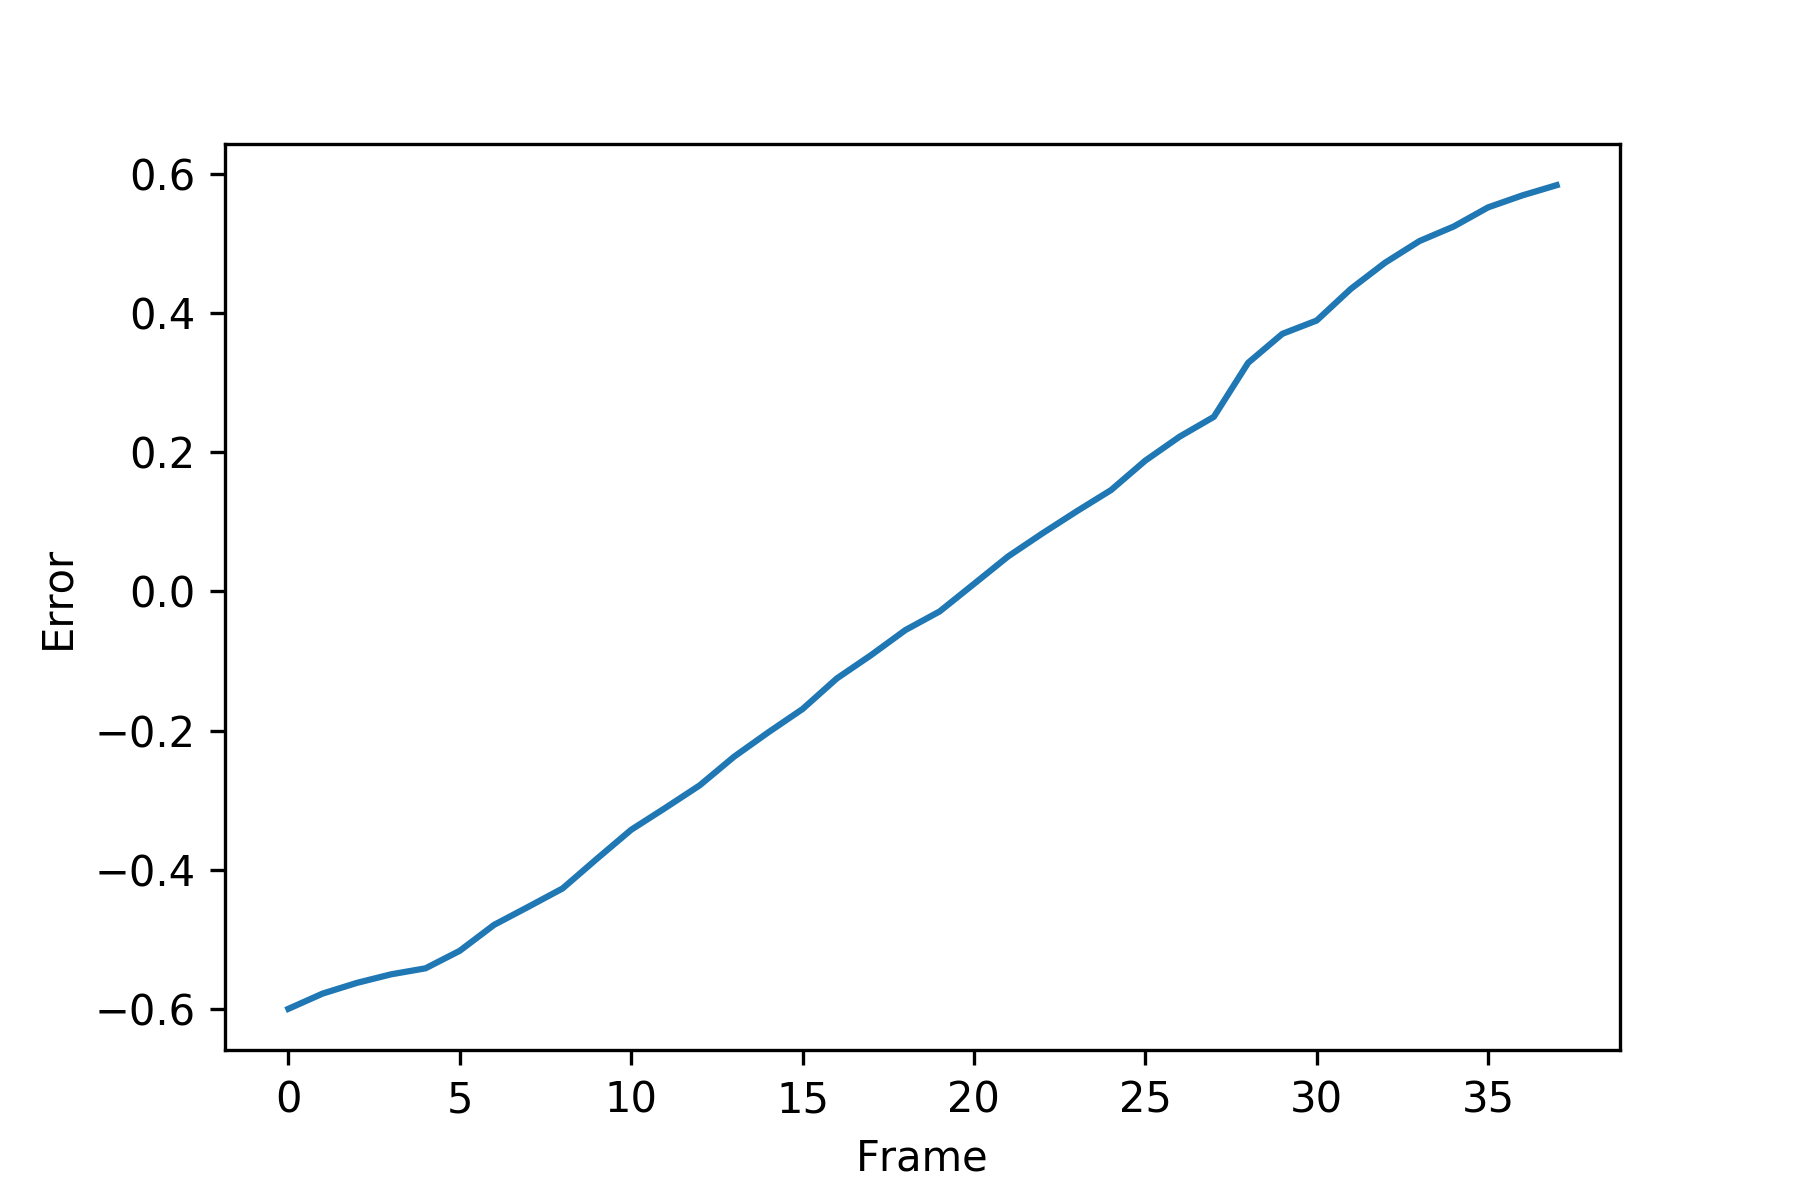
\includegraphics[width=\linewidth]{images/frame_error.png}
\end{center}	
\begin{center}
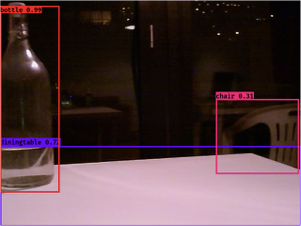
\includegraphics[width=0.31\linewidth]{images/bottle/1}	
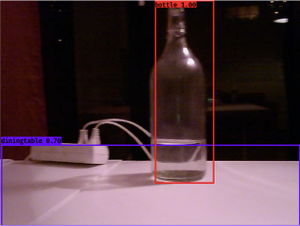
\includegraphics[width=0.31\linewidth]{images/bottle/2}	
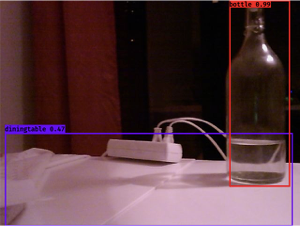
\includegraphics[width=0.31\linewidth]{images/bottle/3}		
\end{center}
\caption{Bounding Box Error}
\end{figure}
The absolute value of the error is bigger when the bottle is on the left or on the right and it is zero when it is in the center of the image. We used it as angular velocity in order to keep the robot pointing to the target object. We make it move forward with a fixed linear velocity of $0.1$.

With these settings we were able to smoothly guide the robot to the target; in the following picture we show some example frame of the moment when the Thymio first sees a \emph{cup} on the left and then moves towards it by keeping it in the middle of its view.
\begin{figure}[H]
\begin{center}
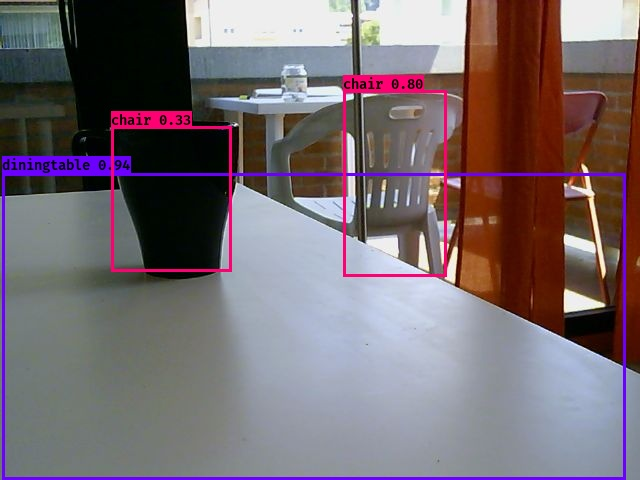
\includegraphics[width=0.48\linewidth]{images/cup/1}	
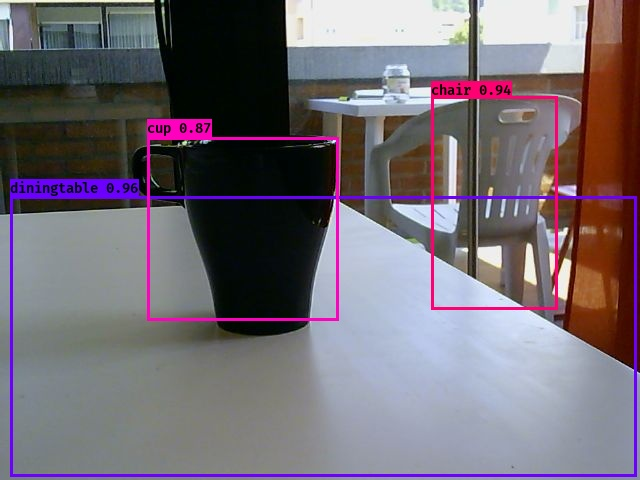
\includegraphics[width=0.48\linewidth]{images/cup/2}	
\end{center}
\begin{center}
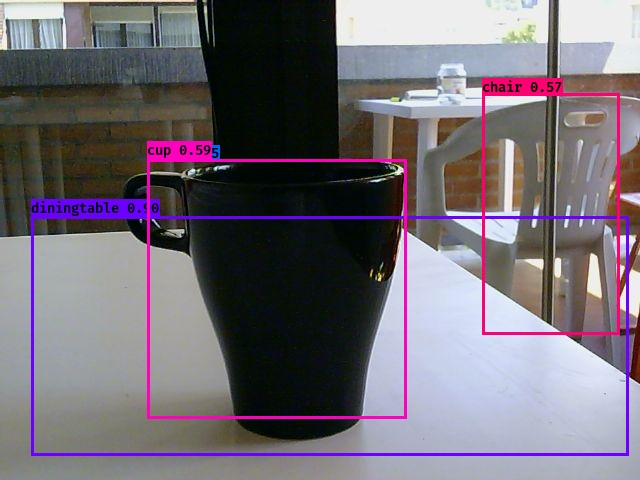
\includegraphics[width=0.48\linewidth]{images/cup/3}	
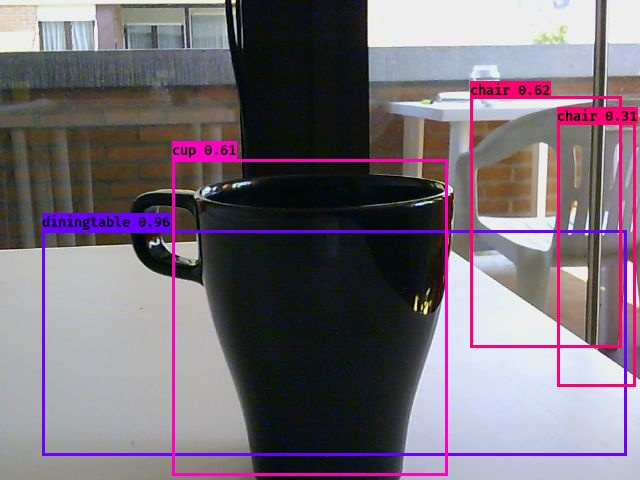
\includegraphics[width=0.48\linewidth]{images/cup/4}	
\end{center}	
\begin{center}
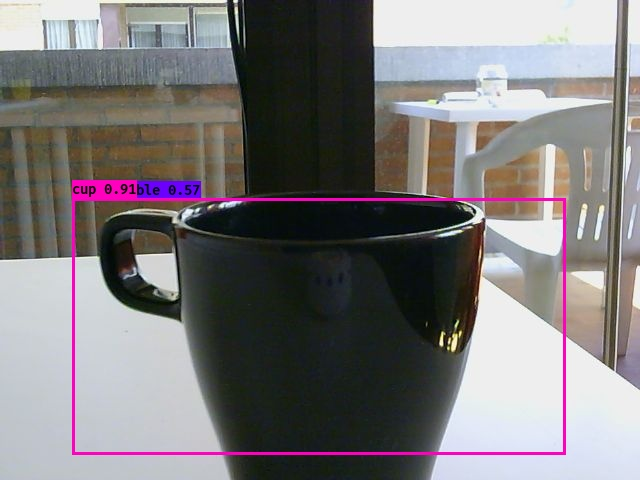
\includegraphics[width=0.48\linewidth]{images/cup/5}	
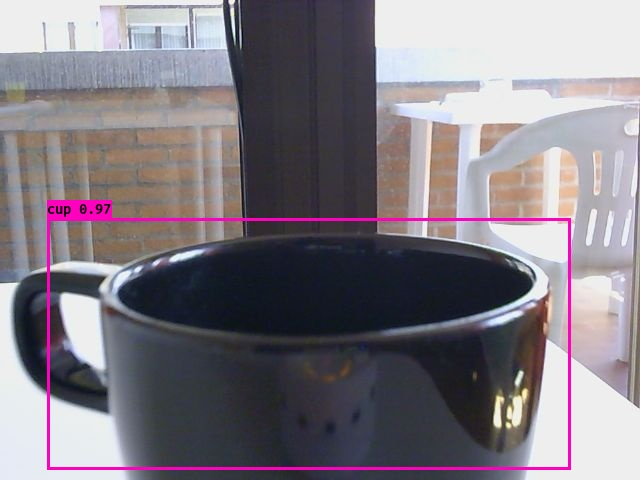
\includegraphics[width=0.48\linewidth]{images/cup/6}	
\end{center}	
\caption{Thymio finds and go to a \emph{cup}}
\end{figure}

\paragraph{Obstacle} When the proximity sensors, five in the front and two in the back, detect something,  the robot stops any activity and goes into the \emph{Obstacle} state. We implemented a simple but yet effective PID controller-based algorithm to move the Thymio away from any object in front or behind it. 

To accomplish this task, we defined two PIDs, one for the linear velocity and one for the angular velocity. The errors are $e_l$ for the linear PID and $e_a$ for the angular PID, defined as follows. We denote the front sensor set as $S_f$ and the rear sensor set as $S_r$, where each element in the set is a double representing the value from the sensor. In our case the cardinality of the sets are $|S_f| = 5$ and $|S_r|=2$.
\begin{align}
	e_l &= \sum\limits_{i=0}^{|S_f|} S_f(i) - \sum\limits_{i = 0}^{|R_f|} R_f(i) \\
	e_a &= (\sum\limits_{i=0}^{\frac{|S_f|}{2}} S_f(i) - \sum\limits_{i = \frac{|S_f|}{2} }^{|S_f|} S_f(i))  \\
	&- (\sum\limits_{i=0}^{\frac{|R_f|}{2}} R_f(i) - \sum\limits_{i = \frac{|R_f|}{2} }^{|R_f|} R_f(i))  \notag
\end{align}
The linear error, $e_l$, is just the sum of all the frontal sensors values minus the rear sensors values.  The angular error is defined as the difference between each pair of sensors on the left and on the right. In both the equations, we subtract the frontal values from the rear ones in order to invert the sign of the PID output so that when there is an obstacle in front of the robot, the velocity is negative and vice-versa. 

As a user feedback, we turn on the five frontal Thymio's LEDs. The number and position of the LEDs are based on the width and the direction of target's bounding box. For example, a big object on the left side will turn on two LEDs, while a smaller object only one. The following figure shows an example where the robot is looking for a \emph{cup}:
\begin{figure}[H]
\begin{center}
	
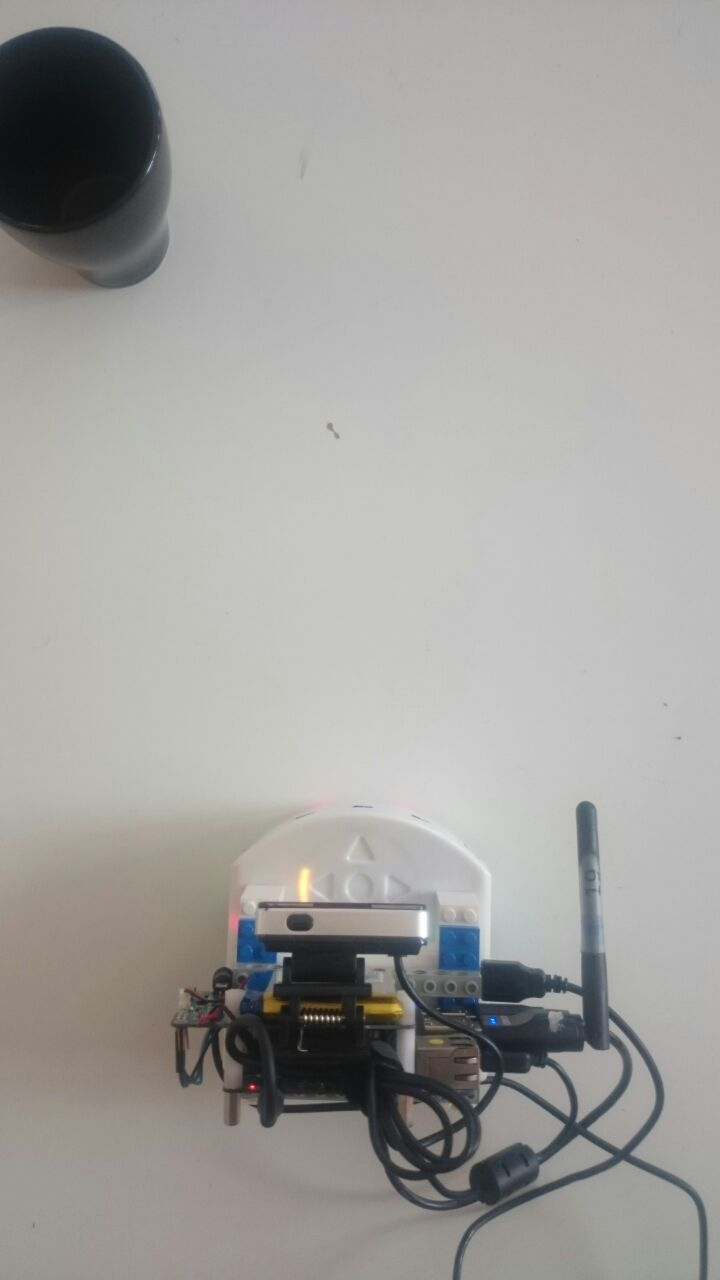
\includegraphics[width=0.25\linewidth]{images/leds/1}	
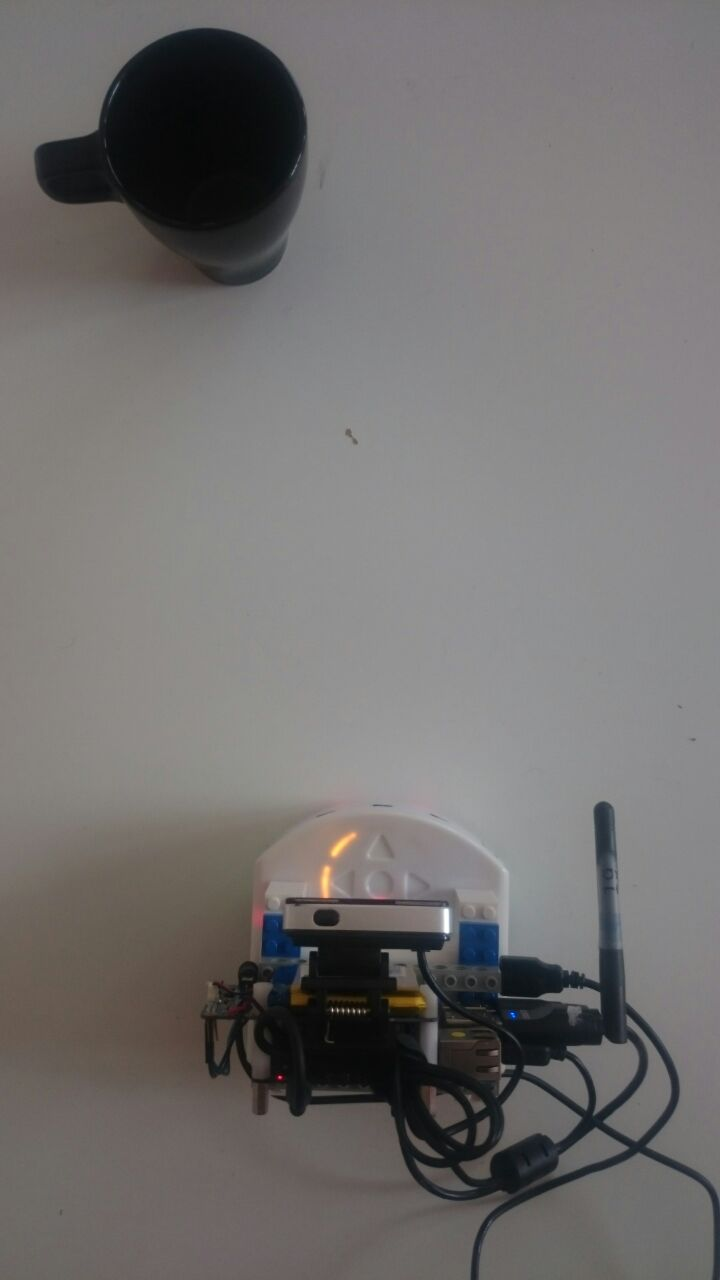
\includegraphics[width=0.25\linewidth]{images/leds/2}	
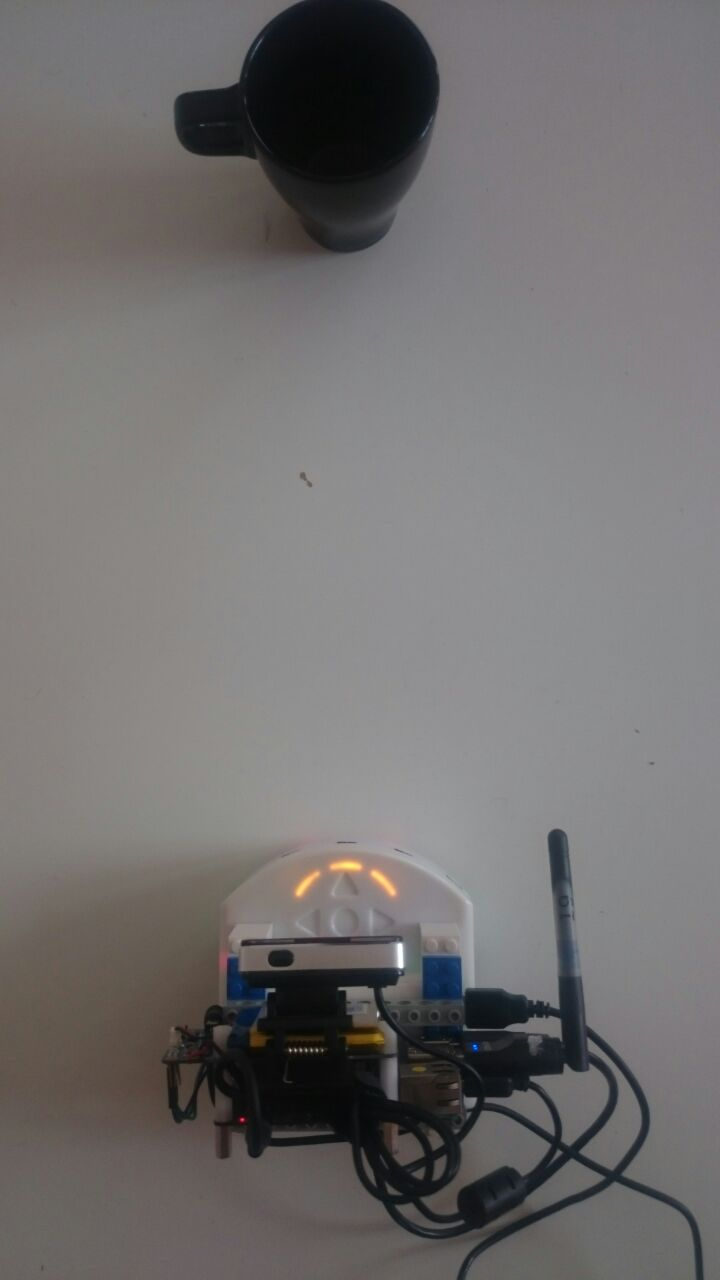
\includegraphics[width=0.25\linewidth]{images/leds/3}	
\end{center}
\begin{center}
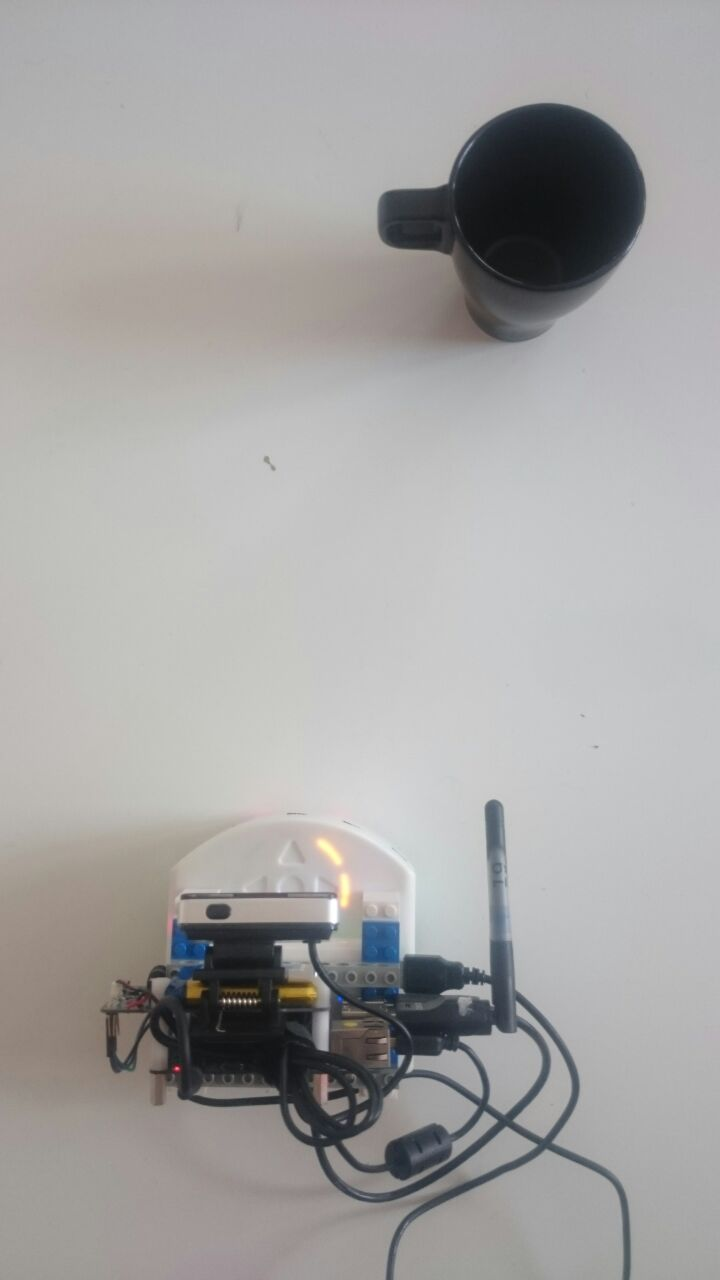
\includegraphics[width=0.25\linewidth]{images/leds/4}	
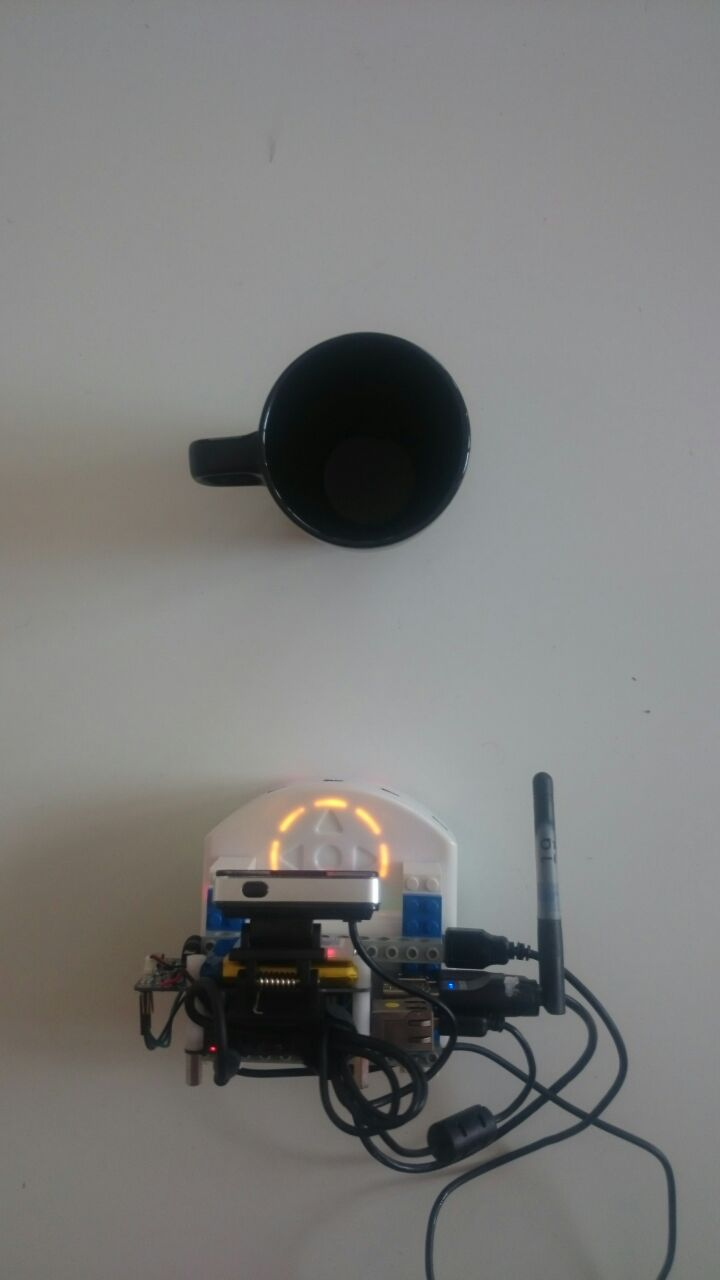
\includegraphics[width=0.25\linewidth]{images/leds/5}
\end{center}
\caption{On board LEDs}
\end{figure}
A video showing the point of view of the Thymio while moving towards a \emph{cup} can be found at 

\section{Conclusion}
In this paper, we presented a light and scalable architecture that uses a real-time Object Detection model to correctly find objects in the surrounding environment and to perform actions based on them. Moreover, because the only  hardware constraint is the camera, our work can be used into similar robots running ROS  to extend their functionalities. Furthermore, since we used YOLO to perform the classification task, the model can be easily re-trained with other classes to increase the context domain. This symbiosis between Machine Learning and Robotics highlights the power of both areas by creating new interesting use cases and scenarios in which both disciplines can shine.

\printbibliography

%\begin{thebibliography}{99}
%%%%%% Our bibliography
%\bibitem{c1} Y. Redmon, S. Divvala, R. Girshick, and A. Farhadi, ÒYou Only Look Once: Unified, Real-Time Object Detection,Ó University of Washington, Allen Institute for AI, Facebook AI Research, May 2016, http://pjreddie.com/yolo/.
%\bibitem{c2} Y. Redmon, and A. Farhadi, ÒYOLOv3: An Incremental Improvement,Ó University of Washington, Apr 2018.
%
%\bibitem{c3} Guzzi, Jérôme and Giusti, Alessandro and Di Caro, Gianni A. and Gambardella, Luca M.,Mighty Thymio for Higher-Level Robotics Education, IDSIA, 2018.

%%%%%  Bibliography templates
%\bibitem{c1} G. O. Young, ÒSynthetic structure of industrial plastics (Book style with paper title and editor),Ó 	in Plastics, 2nd ed. vol. 3, J. Peters, Ed.  New York: McGraw-Hill, 1964, pp. 15Ð64.
%\bibitem{c2} W.-K. Chen, Linear Networks and Systems (Book style).	Belmont, CA: Wadsworth, 1993, pp. 123Ð135.
%\bibitem{c3} H. Poor, An Introduction to Signal Detection and Estimation.   New York: Springer-Verlag, 1985, ch. 4.
%\bibitem{c4} B. Smith, ÒAn approach to graphs of linear forms (Unpublished work style),Ó unpublished.
%\bibitem{c5} E. H. Miller, ÒA note on reflector arrays (Periodical styleÑAccepted for publication),Ó IEEE Trans. Antennas Propagat., to be publised.
%\bibitem{c6} J. Wang, ÒFundamentals of erbium-doped fiber amplifiers arrays (Periodical styleÑSubmitted for publication),Ó IEEE J. Quantum Electron., submitted for publication.
%\bibitem{c7} C. J. Kaufman, Rocky Mountain Research Lab., Boulder, CO, private communication, May 1995.
%\bibitem{c8} Y. Yorozu, M. Hirano, K. Oka, and Y. Tagawa, ÒElectron spectroscopy studies on magneto-optical media and plastic substrate interfaces(Translation Journals style),Ó IEEE Transl. J. Magn.Jpn., vol. 2, Aug. 1987, pp. 740Ð741 [Dig. 9th Annu. Conf. Magnetics Japan, 1982, p. 301].
%\bibitem{c9} M. Young, The Techincal Writers Handbook.  Mill Valley, CA: University Science, 1989.
%\bibitem{c10} J. U. Duncombe, ÒInfrared navigationÑPart I: An assessment of feasibility (Periodical style),Ó IEEE Trans. Electron Devices, vol. ED-11, pp. 34Ð39, Jan. 1959.
%\bibitem{c11} S. Chen, B. Mulgrew, and P. M. Grant, ÒA clustering technique for digital communications channel equalization using radial basis function networks,Ó IEEE Trans. Neural Networks, vol. 4, pp. 570Ð578, July 1993.
%\bibitem{c12} R. W. Lucky, ÒAutomatic equalization for digital communication,Ó Bell Syst. Tech. J., vol. 44, no. 4, pp. 547Ð588, Apr. 1965.
%\bibitem{c13} S. P. Bingulac, ÒOn the compatibility of adaptive controllers (Published Conference Proceedings style),Ó in Proc. 4th Annu. Allerton Conf. Circuits and Systems Theory, New York, 1994, pp. 8Ð16.
%\bibitem{c14} G. R. Faulhaber, ÒDesign of service systems with priority reservation,Ó in Conf. Rec. 1995 IEEE Int. Conf. Communications, pp. 3Ð8.
%\bibitem{c15} W. D. Doyle, ÒMagnetization reversal in films with biaxial anisotropy,Ó in 1987 Proc. INTERMAG Conf., pp. 2.2-1Ð2.2-6.
%\bibitem{c16} G. W. Juette and L. E. Zeffanella, ÒRadio noise currents n short sections on bundle conductors (Presented Conference Paper style),Ó presented at the IEEE Summer power Meeting, Dallas, TX, June 22Ð27, 1990, Paper 90 SM 690-0 PWRS.
%\bibitem{c17} J. G. Kreifeldt, ÒAn analysis of surface-detected EMG as an amplitude-modulated noise,Ó presented at the 1989 Int. Conf. Medicine and Biological Engineering, Chicago, IL.
%\bibitem{c18} J. Williams, ÒNarrow-band analyzer (Thesis or Dissertation style),Ó Ph.D. dissertation, Dept. Elect. Eng., Harvard Univ., Cambridge, MA, 1993. 
%\bibitem{c19} N. Kawasaki, ÒParametric study of thermal and chemical nonequilibrium nozzle flow,Ó M.S. thesis, Dept. Electron. Eng., Osaka Univ., Osaka, Japan, 1993.
%\bibitem{c20} J. P. Wilkinson, ÒNonlinear resonant circuit devices (Patent style),Ó U.S. Patent 3 624 12, July 16, 1990. 

\end{document}
